\begin{figure}[!htb]
  \centering
  \begin{subfigure}[b]{0.4\textwidth}
    \centering
    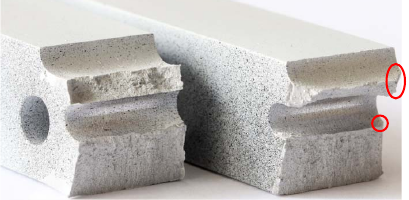
\includegraphics[width=\textwidth,scale=0.5]{Chapter5/figures/3pb/split_experiment}
    \caption{}
  \end{subfigure}
  \begin{subfigure}[b]{0.4\textwidth}
    \centering
    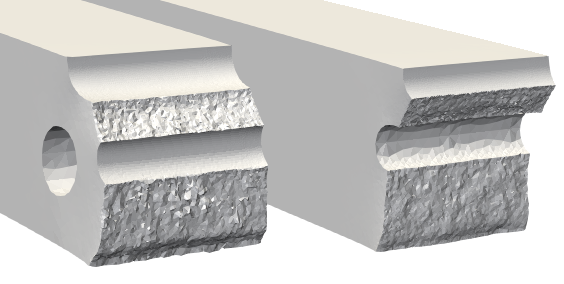
\includegraphics[width=\textwidth,scale=0.5]{Chapter5/figures/3pb/split}
    \caption{}
  \end{subfigure}
  \caption[Comparison of the final crack surfaces between the experiment and the simulation.]{Comparison of the final crack surfaces between (a) the experiment \cite{kubik2019ductile} and (b) the simulation ($\beta = 0.6$ and $\varepsilon_0 = 0.2$). ``Shear lips'' are circled in red. For comparison purposes, the computational domain is separated into two pieces by removing the domain within the $d \ge 0.8$ contour after complete failure.}
  \label{fig: Chapter5/3pb/split_comparison}
\end{figure}
